\documentclass[main.tex]{subfiles}

%\usepackage[]{algorithm2e}
\usepackage{multirow}
\usepackage{algorithmicx}
\usepackage[Algorithm,ruled]{algorithm}
\usepackage{algorithm,algcompatible,amsmath}
\algnewcommand\DESCRIPTION{\item[\textbf{Opis:}]}%
\algnewcommand\INPUT{\item[\textbf{Ulaz:}]}%
\algnewcommand\OUTPUT{\item[\textbf{Izlaz:}]}%

\usepackage{fourier} 
\usepackage{array}
\usepackage{makecell}
\renewcommand\theadalign{cc}
\renewcommand\theadfont{\bfseries}
\renewcommand\theadgape{\Gape[4pt]}
\renewcommand\cellgape{\Gape[4pt]}

\usepackage{amsmath,bm}
\usepackage{adjustbox}

\usepackage[demo]{graphicx}
\usepackage{caption}
\usepackage{subcaption}

%\usepackage{lmodern}
%\usepackage{siunitx}
%\usepackage{booktabs}
%\usepackage{etoolbox}

\usepackage{lscape} 

% for avoiding siunitx using bold extended
%\renewrobustcmd{\bfseries}{\fontseries{b}\selectfont}
%\renewrobustcmd{\boldmath}{}
% abbreviation
%\newrobustcmd{\B}{\bfseries}


\begin{document}

U ovom poglavlju će biti izloženi eksperimentalni rezultati predstavljenih metoda za rešavanje simboličke regresije. Sva testiranja su izvršena na računaru sa Intel Core i7 procesorom od 16GB i SSD-om, a sve metode su implementirane u programskom jeziku Python.

\subsection{Podaci}
\label{sec:data}

Predstavljene metode su testirane pomoću tri vrste skupova podataka. 

%Jedanu vrstu skupa čine slučajno generisane instance 
Jedna vrsta skupova je generisana na osnovu funkcija koje se često razmatraju u literaturi \cite{vnp}, \cite{semanticCrossover}, \cite{beeColony}. Instance ovog skupa su generisane na osnovu slučajno odabranih vrednosti nezavisnih promenljiih. Za svaku funkciju je generisano 100 instanci. Funkcije i intervali vrednosti iz kojeg su birane tačke su:

$ F_1 = x^3 + x^2 + x, \quad x \in [-1, 1] $

$ F_2 = x^4 + x^3 + x^2 + x, \quad x \in [-1, 1] $

$ F_3 = x^5 + x^4 + x^3 + x^2 + x, \quad x \in [-1, 1] $

$ F_4 = x^6 + x^5 + x^4 + x^3 + x^2 + x, \quad x \in [-1, 1] $

$ F_5 = sin(x^2)cos(x) - 1, \quad x \in [-1, 1] $

$ F_6 = sin(x) + sin(x + x^2), \quad x \in [-1, 1] $

$ F_7 = log(x + 1) + log(x^2 + 1), \quad x \in [0, 2] $

$ F_8 = sin(x_0) + sin(x_1^2), \quad x_0, x_1 \in [-1, 1] $

$ F_9 = 2sin(x_0)cos(x_1), \quad x_0, x_1 \in [-1, 1] $



Drugu vrstu testa čini evaluacija implementiranih metoda nad nekim od javno dostupnih skupova podataka za regresiju. Ovde je iskorišćen "Yacht Hydrodynamics" skup \cite{datasetYacht}, kod koga je cilj predvideti vrednost rezidualnog otpora jahte na osnovu njenih karakteristika. Skup sadrži 308 instanci koje su određene pomoću 6 nezavisnih i jedne ciljne promenljive. Sve vrednosti su realnog tipa.

Dodatno, generisani su i skupovi podataka na osnovu nekih jednostavnijih funkcija koje su uzete radi upoređivanja metaheurističkih metoda sa metodom grube sile, jer metoda grube sile nije mogla uspešno da se nađe tačno rešenje na velikom broju prethodno pomenutih skupova. Te funkcije su:

$F_{01} = x_0 x_1 + x_1$

$F_{02} = x_1 + x_1^2 + x_0$

$F_{03} = x_0 x_1 + cos(x_0)$

$F_{04} = x_0 - x_1 x_1$

$F_{05} = x_0 - x_1 x_1 + x_1$


\subsection{Evaluacija algoritma grube sile i poređenje sa metaheurističkim metodama}
\label{sec:bruteForceEval}

Algoritam grube sile je uspešno mogao da dođe do optimalnog rešenja za primere $F_{01}, ..., F_{05}$ i $F_{1}$ i $F_{2}$. U ostalim slučajevima je, nakon više sati izvršavanja, dolazilo do nedostatka memorijskih resursa, bez pronalaska dovoljno dobrog rešenja.

Svi metaheuristički pristupi su, takođe, uspešno pronašli optimalno rešenje za primere $F_{01}, ..., F_{05}$. U tabeli \ref{tbl:bruteForceResults} je prikazano vreme izvršavanja koje je u proseku bilo potrebno svakoj od metoda za pronalazak ciljne funkcije. Kolone tabele predstavljaju metode, a redovi funkcije. U preseku $i$-te vrste i $j$-te kolone je prikazano vreme izvršavanja (izraženo u sekundama) $j$-te metode nad instancama $i$-te funkcije.


\iffalse

\begin{table}
\caption{Vreme izvršavanja svih metoda na poblemima manjih dimenzija}
\label{tbl:bruteForceResults}
\begin{center}
\begin{tabular}{ |c|c|c|c| } 
\hline
\thead{Metoda} & \thead{Funkcija / \\ Skup \\ podataka} & \thead{Vreme izvršavanja (H:M:S)} \\
\hline
\multirow{7}{*}{Algoritam grube sile} 
& $F_{01}$ & 00:00:01 \\ 
& $F_{02}$ & 00:00:00 \\ 
& $F_{03}$ & 00:00:00 \\ 
& $F_{04}$ & 00:00:00 \\
& $F_{05}$ & 00:00:00 \\
& $F_{1}$ & 00:00:00 \\
& $F_{2}$ & 00:00:22\\
\hline
\multirow{7}{*}{GP} 
& $F_{01}$ & 00:00:12 \\ 
& $F_{02}$ & 00:00:07 \\ 
& $F_{03}$ & 00:00:06 \\ 
& $F_{04}$ & 00:00:12 \\
& $F_{05}$ & 00:00:07 \\
& $F_{1}$ & 00:00:15 \\
& $F_{2}$ & 00:00:13 \\
\hline
\multirow{7}{*}{GP sa SSC} 
& $F_{01}$ & 00:00:19 \\ 
& $F_{02}$ & 00:00:13 \\ 
& $F_{03}$ & 00:00:12 \\ 
& $F_{04}$ & 00:00:18 \\
& $F_{05}$ & 00:00:18 \\
& $F_{1}$ & 00:00:24 \\
& $F_{2}$ & 00:00:26 \\
\hline
\multirow{7}{*}{VNP} 
& $F_{01}$ & 00:00:04 \\ 
& $F_{02}$ & 00:00:06 \\ 
& $F_{03}$ & 00:00:06 \\ 
& $F_{04}$ & 00:00:05 \\
& $F_{05}$ & 00:00:06 \\
& $F_{1}$ & 00:00:07 \\
& $F_{2}$ & 00:00:08 \\
\hline
\end{tabular}
\end{center}
\end{table}

\fi


\begin{table}
\caption{Vreme izvršavanja (izraženo u sekundama) svih metoda na poblemima manjih dimenzija}
\label{tbl:bruteForceResults}
\begin{center}
\begin{tabular}{ |c|c|c|c|c| } 
\hline
\thead{} & \thead{Algoritam \\ grube sile} & \thead{GP} & \thead{GP sa SSC} & \thead{VNP} \\
\hline
$\boldsymbol F_{\boldsymbol 0 \boldsymbol 1}$ & 1 & 12 & 19 & 4 \\ 
\hline
$\boldsymbol F_{\boldsymbol 0 \boldsymbol 2}$ & <1 & 7 & 13 & 6 \\ 
\hline
$\boldsymbol F_{\boldsymbol 0 \boldsymbol 3}$ & <1 & 6 & 12 & 6 \\ 
\hline
$\boldsymbol F_{\boldsymbol 0 \boldsymbol 4}$ & <1 & 12 & 18 & 5 \\ 
\hline
$\boldsymbol F_{\boldsymbol 0 \boldsymbol 5}$ & <1 & 7 & 18 & 6 \\ 
\hline
$\boldsymbol F_{\boldsymbol 1}$ & <1 & 15 & 24 & 7 \\ 
\hline
$\boldsymbol F_{\boldsymbol 2}$ & 22 & 13 & 26 & 8 \\ 
\hline
\end{tabular}
\end{center}
\end{table}

\subsection{Evaluacija i poređenje metaheurističkih metoda}
\label{sec:metaheuristicsEval}

U ovoj sekciji će biti predstavljeni i međusobno upoređeni rezultati metaheurističkih metoda.

Kada je problem simboličke regresije tek počeo da se rešava, efikasnost metoda je predstavljana u terminima koji odgovaraju metaheuristikama \cite{semanticCrossover}, \cite{beeColony}. Na primer, jedan način za evaluaciju tačnosti je bio na osnovu srednje vrednosti najboljih vrednosti funkcija prilagođenosti dobijenih pri većem broju nezavisnih pokretanja programa. Drugi način se definisao na osnovu broja uspešnih pokretanja od ukupnog broja pokretanja programa, gde se pod uspešnim pokretanjem smatralo ono u kom postoji barem jedna jedinka koja za svaku instancu iz skupa podataka daje grešku manju od nekog definisanog praga.

Poslednjih godina metode za simboličku regresiju se evaluiraju kao i metode za sve druge tipove regresije \cite{GPIncompleteData}, \cite{linearScalingGP}, \cite{benchmarkStudy}. To podrazumeva podelu skupa podataka na trening i test deo i evaluaciju dobijenog modela pomoću MSE, RMSE, $R^2$ i sličnih metrika. U ovom radu je primenjen ovaj pristup. Za trening je uzeto 70\% podataka, za test 30\% , a evaluacija je urađena pomoću $R^2$ koeficijenta određenosti. Veće $R^2$ vrednosti odgovaraju izrazima koji su bliži optimalnom. Optimalnim izrazom smatraće se i onaj izraz koji originalno ima različit simbolički zapis od ciljnog izraza, ali nakon algebarske simplifikacije dobija njegovu strukturu. Odnosno, ako za ciljni izraz $f$ i nađeni izraz $f'$ važi da algebarska simplifikacija izraza $f' - f$ daje simbol "0", biće smatrano da je pronađeno optimalno rešenje. Za proces algebarskog pojednostavljivanja je korišćen SymPy paket \cite{sympy}.

Svaka metoda je evaluirana tako što je pokrenuta po 30 puta nad svim skupovima podataka. Prilikom svakog od tih nezavisnih pokretanja dobijen je izraz koji u tom izvršavanju najbolje odgovara datom skupu podataka. Za taj izraz je zatim izračunat koeficijent određenosti na trening i test skupu i provereno je da li i simbolički odgovara ciljnom izrazu po postupku koji je naveden iznad. Naravno, provera optimalnosti u simboličkom smislu je rađena samo za skupove podataka kod kojih je poznata ciljna funkcija. Kod "Yacht Hydrodynamics" skupa taj deo je izostavljen. Takođe, pri svakom pokretanju mereno je i vreme koje je bilo potrebno za pronalazak najboljeg rešenja.

U tabeli \ref{tbl:gpParameters} su prikazane vrednosti koje su korišćene za parametre genetskog programiranja. Odabrane su zbog čestog korišćenja u radovima koji se bave rešavanjem ovog problema pomoću genetskog programiranja i na osnovu dobrih rezultata pri inicijalnom testianju metode.
Kod "Yacht" skupa je bilo potrebno povećati dozvoljenu veličinu populacije i veličinu jedinki. Parametri koišćeni za ovaj skup se mogu videti u tabeli \ref{tbl:gpParametersYacht}. 

\begin{table}[ht]
\caption{Vrednosti parametara genetskog programiranja} 
\label{tbl:gpParameters}
\centering
\begin{tabular}{l l} % centered columns (4 columns)
\hline 
Parametar & Vrednost \\ [0.5ex] 
\hline 
Veličina populacije & 500  \\ 
Maksimalan broj generacija & 50  \\
Broj jedinki za reprodukciju & 300  \\
Veličina turnira & 3 \\
Verovatnoća mutacie pojedinačnog čvora & 0.2  \\
Verovatnoća mutacije celog podstabla & 0.2  \\ 
Minimalna dubina stabla & 2 \\
Maksimalna dubina stabla u fazi inicijalizacije & 6 \\
Maksimalna veličina stabla & 16 \\
Vrsta funkcije prilagođenosti & adjusted \\ 
Skup funkcija &  +, -, *, /, pow, sin, cos, log \\ [1ex] % [1ex] adds vertical space
\hline 
\end{tabular}
\end{table}


\begin{table}[ht]
\caption{Vrednosti parametara genetskog programiranja za "Yacht Hydrodynamics" skup podataka} 
\label{tbl:gpParametersYacht}
\centering
\begin{tabular}{l l} % centered columns (4 columns)
\hline 
Parametar & Vrednost \\ [0.5ex] 
\hline 
Veličina populacije & 2000  \\ 
Maksimalan broj geneacija & 100  \\
Broj jedinki za reprodukciju & 1200  \\
Veličina turnira & 10 \\
Verovatnoća mutacie pojedinačnog čvora & 0.2  \\
Verovatnoća mutacije celog podstabla & 0.2  \\ 
Minimalna dubina stabla & 2 \\
Maksimalna dubina stabla u fazi inicijalizacije & 12 \\
Maksimalna veličina stabla & 64 \\
Vrsta funkcije prilagođenosti & adjusted \\ 
Skup funkcija &  +, -, *, /, pow, sin, cos, log \\ [1ex] % [1ex] adds vertical space
\hline 
\end{tabular}
\end{table}


U tabeli \ref{tbl:vnpParameters} se mogu videti korišćene vrednosti parametara za metodu promenljivih okolina na svim skupovima podataka, osim za "Yacht". Kod njega je za $k_{max}$ uzeta vrednost 6, a broj iteracija je povećan na 2000.


\begin{table}[H]
\caption{Vrednosti parametara metode promenljivih okolina} 
\label{tbl:vnpParameters}
\centering
\begin{tabular}{l l} % centered columns (4 columns)
\hline 
Parametar & Vrednost \\ [0.5ex] 
\hline 
$k_{max}$ & 4  \\ 
Minimalna dubina stabla & 2 \\
Maksimalna dubina stabla u fazi inicijalizacije & 4 \\
Maksimalna dubina stabla kreiranog u fazi prerage  & 6 \\
Maksimalan broj iteracija & 1000 \\ 
Skup funkcija &  +, -, *, /, pow, sin, cos, log \\ [1ex] % [1ex] adds vertical space
\hline 
\end{tabular}
\end{table}
\clearpage

\iffalse
\begin{table}
\caption{Prosečne vrednosti određenih karakteristika u 30 nezavisnih pokretanja}
\label{tbl:meanVals1}
\begin{center}
\begin{tabular}{ |c|c|c|c|c|c|c| } 
\hline
\thead{Metoda} & \thead{Funkcija / \\ Skup \\ podataka} & \thead{Prosečna \bm{$R^2$} \\ vrednost na \\ trening skupu} & \thead{Prosečna \bm{$R^2$} \\ vrednost na \\ test skupu} & \thead{Broj \\ pokretanja \\ u kojima je \\ pronađeno rešenje \\ simbolički ekvivalentno \\ ciljnom rešenju} &  \thead{Prosečno \\ vreme \\ izvršavanja \\ (s)} \\
\hline
\multirow{5}{*}{GP} 
& $F_{01}$ & 0.879 & 0.898 & 7 & 12 \\
& $F_{02}$ & 0.765 & 0.791 & 1 & 7 \\
& $F_{03}$ & 0.745 & 0.810 & 5 & 6\\
& $F_{04}$ & 0.773 & 0.820 & 2 & 12 \\
& $F_{05}$ & 0.795 & 0.797 & 3 & 7 \\
\hline
\multirow{5}{*}{GP sa SSC}
& $F_{01}$ & 0.831 & 0.861 & 3 & 19  \\
& $F_{02}$ & 0.802 & 0.818 & 3 & 13 \\
& $F_{03}$ & 0.733 & 0.820 & 5 & 12 \\
& $F_{04}$ & 0.740 & 0.775 & 1 & 18 \\
& $F_{05}$ & 0.771 & 0.765 & 1 & 18 \\
\hline
\multirow{5}{*}{VNP} 
& $F_{01}$ & 0.949 & 0.945 & 13 & 4 \\
& $F_{02}$ & 0.848 & 0.897 & 11 & 6 \\
& $F_{03}$ & 0.863 & 0.926 & 14 & 5 \\
& $F_{04}$ & 0.914 & 0.922 & 9 & 5 \\
& $F_{05}$ & 0.846 & 0.813 & 9 & 7 \\
\hline
\end{tabular}
\end{center}
\end{table}
\fi

\begin{landscape}
\newcolumntype{?}{!{\vrule width 1pt}}
\begin{table}
\caption{Prosečne vrednosti određenih karakteristika u 30 nezavisnih pokretanja}
\label{tbl:meanVals1}
\begin{center}
\begin{tabular}{ |c?|c|c|c?|c|c|c?|c|c|c?|c|c|c| } 
\hline
& \multicolumn{3}{|c?|}{\thead{Prosečna \bm{$R^2$} vrednost \\ na  trening skupu}} & \multicolumn{3}{|c?|}{\thead{Prosečna \bm{$R^2$} vrednost \\ na test skupu}} & \multicolumn{3}{|c?|}{\thead{Broj pokretanja u kojima je \\ pronađeno rešenje \\ simbolički ekvivalentno \\ ciljnom rešenju}} & \multicolumn{3}{|c|}{\thead{Prosečno vreme \\ izvršavanja (s)}}  \\
\hline
& \textbf{GP} & \textbf{GP sa SSC} & \textbf{VNP} & \textbf{GP} & \textbf{GP sa SSC} & \textbf{VNP} & \textbf{GP} & \textbf{GP sa SSC} & \textbf{VNP} & \textbf{GP} & \textbf{GP sa SSC} & \textbf{VNP} \\
\hline
$\boldsymbol F_{\boldsymbol 0 \boldsymbol 1}$ & 0.879 & 0.831 & \textbf{0.949} & 0.898 & 0.861 & \textbf{0.945} & 7 & 3 & \textbf{13} & 12 & 19 & \textbf{4} \\
\hline
$\boldsymbol F_{\boldsymbol 0 \boldsymbol 2}$ & 0.765 & 0.802 & \textbf{0.848} & 0.791 & 0.818 & \textbf{0.897} & 1 & 3 & \textbf{11} & 7 & 13 & \textbf{6} \\
\hline
$\boldsymbol F_{\boldsymbol 0 \boldsymbol 3}$ & 0.745 & 0.733 & \textbf{0.863} & 0.810 & 0.820 & \textbf{0.926} & 5 & 5 & \textbf{14} & 6 & 12 & \textbf{5} \\
\hline
$\boldsymbol F_{\boldsymbol 0 \boldsymbol 4}$ & 0.733 & 0.740 & \textbf{0.914} & 0.820 & 0.775 & \textbf{0.922} & 2 & 1 & \textbf{9} & 12 & 18 & \textbf{5} \\
\hline
$\boldsymbol F_{\boldsymbol 0 \boldsymbol 5}$ & 0.795 & 0.771 & \textbf{0.846} & 0.797 & 0.765 & \textbf{0.813} & 3 & 1 & \textbf{9} & \textbf{7} & 18 & \textbf{7} \\
\hline
\end{tabular}
\end{center}
\end{table}
\end{landscape}


\iffalse
\begin{table}
\caption{Prosečne vrednosti određenih karakteristika u 30 nezavisnih pokretanja}
\label{tbl:meanVals2}
\begin{center}
\begin{tabular}{ |c|c|c|c|c|c|c| } 
\hline
\thead{Metoda} & \thead{Funkcija / \\ Skup \\ podataka} & \thead{Prosečna \bm{$R^2$} \\ vrednost na \\ trening skupu} & \thead{Prosečna \bm{$R^2$} \\ vrednost na \\ test skupu} & \thead{Broj \\ pokretanja \\ u kojima je \\ pronađeno rešenje \\ simbolički ekvivalentno \\ ciljnom rešenju} &  \thead{Prosečno \\ vreme \\ izvršavanja \\ (H:M:S)} \\
\hline
\multirow{7}{*}{GP} 
& $F_{1}$ & 0.914 & 0.907 & 0 & 00:00:15 \\
& $F_{2}$ & 0.827 & 0.824 & 0 & 00:00:13 \\
& $F_{3}$ & 0.851 & 0.695 & 0 & 00:00:20 \\
& $F_{4}$ & 0.746 & 0.796 & 0 & 00:00:14 \\
& $F_{5}$ & 0.643 & 0.607 & 0 & 00:00:14 \\
& $F_{6}$ & 0.928 & 0.883 & 0 & 00:00:13 \\
& $F_{7}$ & 0.960 & 0.950 & 0 & 00:00:18 \\
& $F_{8}$ & 0.857 & 0.716 & 0 & 00:00:13 \\
& $F_{9}$ & 0.950 & 0.955 & 1 & 00:00:12 \\
\hline
\multirow{7}{*}{GP sa SSC}
& $F_{1}$ & 0.861 & 0.827 & 0 & 00:00:24 \\
& $F_{2}$ & 0.799 & 0.798 & 0 & 00:00:26 \\
& $F_{3}$ & 0.851 & -1.428 & 0 & 00:00:23 \\
& $F_{4}$ & 0.691 & 0.743 & 0 & 00:00:27 \\
& $F_{5}$ & 0.606 & 0.589 & 0 & 00:00:24 \\
& $F_{6}$ & 0.917 & 0.881 & 0 & 00:00:27 \\
& $F_{7}$ & 0.968 & 0.959 & 0 & 00:00:51 \\
& $F_{8}$ & 0.837 & 0.657 & 0 & 00:00:35 \\
& $F_{9}$ & 0.940 & 0.938 & 1 & 00:00:28 \\
\hline
\multirow{7}{*}{VNP} 
& $F_{1}$ & 0.907 & 0.872 & 13 & 00:00:07 \\
& $F_{2}$ & 0.771 & 0.770 & 9 & 00:00:09 \\
& $F_{3}$ & 0.797 & 0.752 & 2 & 00:00:10 \\
& $F_{4}$ & 0.809 & 0.778 & 2 & 00:00:12 \\
& $F_{5}$ & 0.894 & 0.887 & 0 & 00:00:14 \\
& $F_{6}$ & 0.945 & 0.930 & 1 & 00:00:12 \\
& $F_{7}$ & 0.994 & 0.993 & 0 & 00:00:13 \\
& $F_{8}$ & 0.968 & 0.936 & 3 & 00:00:07 \\
& $F_{9}$ & 0.963 & 0.971 & 2 & 00:00:08 \\
\hline
\end{tabular}
\end{center}
\end{table}
\fi 

\begin{landscape}
\newcolumntype{?}{!{\vrule width 1pt}}
\begin{table}
\caption{Prosečne vrednosti određenih karakteristika u 30 nezavisnih pokretanja}
\label{tbl:meanVals2}
\begin{center}
\begin{tabular}{ |c?|c|c|c?|c|c|c?|c|c|c?|c|c|c| } 
\hline
& \multicolumn{3}{|c?|}{\thead{Prosečna \bm{$R^2$} vrednost \\ na  trening skupu}} & \multicolumn{3}{|c?|}{\thead{Prosečna \bm{$R^2$} vrednost \\ na test skupu}} & \multicolumn{3}{|c?|}{\thead{Broj pokretanja u kojima je \\ pronađeno rešenje \\ simbolički ekvivalentno \\ ciljnom rešenju}} & \multicolumn{3}{|c|}{\thead{Prosečno vreme \\ izvršavanja (s)}}  \\
\hline
& \textbf{GP} & \textbf{GP sa SSC} & \textbf{VNP} & \textbf{GP} & \textbf{GP sa SSC} & \textbf{VNP} & \textbf{GP} & \textbf{GP sa SSC} & \textbf{VNP} & \textbf{GP} & \textbf{GP sa SSC} & \textbf{VNP} \\
\hline
$\boldsymbol F_{\boldsymbol 1}$ & \textbf{0.914} & 0.861 & 0.907 & \textbf{0.907} & 0.827 & 0.872 & 0 & 0 & \textbf{13} & 15 & 24 & \textbf{7} \\
\hline
$\boldsymbol F_{\boldsymbol 2}$ & \textbf{0.827} & 0.799 & 0.771 & \textbf{0.824} & 0.798 & 0.770 & 0 & 0 & \textbf{9} & 13 & 26 & \textbf{9} \\
\hline
$\boldsymbol F_{\boldsymbol 3}$ & \textbf{0.851} & 0.851 & 0.797 & 0.695 & -1.428 & \textbf{0.752} & 0 & 0 & \textbf{2} & 20 & 23 & \textbf{10} \\
\hline
$\boldsymbol F_{\boldsymbol 4}$ & 0.746 & 0.691 & \textbf{0.809} & \textbf{0.796} & 0.743 & 0.778 & 0 & 0 & \textbf{2} & 14 & 27 & \textbf{12} \\
\hline
$\boldsymbol F_{\boldsymbol 5}$ & 0.643 & 0.606 & \textbf{0.894} & 0.607 & 0.589 & \textbf{0.887} & 0 & 0 & 0 & \textbf{14} & 24 & \textbf{14} \\
\hline
$\boldsymbol F_{\boldsymbol 6}$ & 0.928 & 0.917 & \textbf{0.945} & 0.883 & 0.881 & \textbf{0.930} & 0 & 0 & \textbf{1} & 13 & 27 & \textbf{12} \\
\hline
$\boldsymbol F_{\boldsymbol 7}$ & 0.960 & 0.968 & \textbf{0.994} & 0.950 & 0.959 & \textbf{0.993} & 0 & 0 & 0 & 18 & 51 & \textbf{13} \\
\hline
$\boldsymbol F_{\boldsymbol 8}$ & 0.857 & 0.837 & \textbf{0.968} & 0.716 & 0.657 & \textbf{0.936} & 0 & 0 & \textbf{3} & 13 & 35 & \textbf{7} \\
\hline
$\boldsymbol F_{\boldsymbol 9}$ & 0.950 & 0.940 & \textbf{0.963} & 0.955 & 0.938 & \textbf{0.971} & 1 & 1 & \textbf{2} & 12 & 28 & \textbf{8} \\
\hline
\end{tabular}
\end{center}
\end{table}
\end{landscape}



\begin{table}
\caption{Prosečne vrednosti određenih karakteristika u 30 nezavisnih pokretanja za "Yacht Hydrodynamics" skup podataka}
\label{tbl:meanVals3}
\begin{center}
\begin{tabular}{ |c|c|c|c|c| } 
\hline
\thead{Metoda} & \thead{Prosečna \bm{$R^2$} \\ vrednost na \\ trening skupu} & \thead{Prosečna \bm{$R^2$} \\ vrednost na \\ test skupu} &  \thead{Prosečno vreme \\ izvršavanja (s)} \\
\hline
\multirow{1}{*}{GP} 
& 0.238 & 0.264 & 183 \\
\hline
\multirow{1}{*}{GP sa SSC}
& 0.213 & 0.233 & 247  \\
\hline
\multirow{1}{*}{VNP} 
& \textbf{0.477} & \textbf{0.457} & \textbf{30} \\
\hline
\end{tabular}
\end{center}
\end{table}


\iffalse
\begin{table}
\caption{Informacije o izrazu koji daje maksimalnu $R^2$ vrednost na test skupu od svih izraza dobijenih pri 30 nezavisnih pokretanja}
\label{tbl:maxVals1}
\begin{center}
\begin{tabular}{ |c|c|c|c|c|c| } 
\hline
\thead{Metoda} & \thead{Funkcija / \\ Skup \\ podataka} & \thead{Maksimalna \bm{$R^2$} \\ vrednost na \\ test skupu} & \thead{Izraz koji ima \\ maksimalnu \bm{$R^2$} \\ vrednost na \\ test skupu } & \thead{Simbolička ekvivalencija \\ sa ciljnim izrazom} \\
\hline
\multirow{5}{*}{GP} 
& $F_{01}$ & 1.0 & $x_1(x_0 + 1)$ & Da \\
& $F_{02}$ & 1.0 & $x_0 + x_1^2 + x_1$ & Da \\
& $F_{03}$ & 1.0 & $x_0 x_1 + cos(x_0)$ & Da \\
& $F_{04}$ & 1.0 & $x_0 - x_1^2$ & Da \\
& $F_{05}$ & 1.0 & $x_0 - x_1^2 + x_1$ & Da \\
\hline
\multirow{5}{*}{GP sa SSC}
& $F_{01}$ & 1.0 & $x_1(x_0 + 1)$ & Da \\
& $F_{02}$ & 1.0 & $x_0 + x_1^2 + x_1$ & Da \\
& $F_{03}$ & 1.0 & $x_0 x_1 + cos(x_0)$ & Da \\
& $F_{04}$ & 1.0 & $x_0 - x_1^2$ & Da \\
& $F_{05}$ & 1.0 & $x_0 - x_1^2 + x_1$ & Da \\
\hline
\multirow{5}{*}{VNP} 
& $F_{01}$ & 1.0 & $x_1(x_0 + 1)$ & Da \\
& $F_{02}$ & 1.0 & $x_0 + x_1^2 + x_1$ & Da \\
& $F_{03}$ & 1.0 & $x_0 x_1 + cos(x_0)$ & Da \\
& $F_{04}$ & 1.0 & $x_0 - x_1^2$ & Da \\
& $F_{05}$ & 1.0 & $x_0 - x_1^2 + x_1$ & Da \\
\hline
\end{tabular}
\end{center}
\end{table}
\fi


\begin{landscape}
\newcolumntype{?}{!{\vrule width 1pt}}
\begin{table}
\caption{Informacije o izrazu koji daje maksimalnu $R^2$ vrednost na test skupu od svih izraza dobijenih pri 30 nezavisnih pokretanja}
\label{tbl:maxVals1}
\begin{center}
\begin{tabular}{ |c?|c|c|c?|c|c|c?|c|c|c| } 
\hline
& \multicolumn{3}{|c?|}{\thead{Maksimalna \bm{$R^2$} vrednost \\ na  test skupu}} & \multicolumn{3}{|c?|}{\thead{Izraz koji ima maksimalnu \\ \bm{$R^2$} vrednost na test skupu}} & \multicolumn{3}{|c|}{\thead{Simbolička \\ ekvivalencija sa \\ ciljnim izrazom}} \\
\hline
& \textbf{GP} & \textbf{GP sa SSC} & \textbf{VNP} & \textbf{GP} & \textbf{GP sa SSC} & \textbf{VNP} & \textbf{GP} & \textbf{GP sa SSC} & \textbf{VNP} \\
\hline
$\boldsymbol F_{\boldsymbol 0 \boldsymbol 1}$ & 1.0 & 1.0 & 1.0 & $x_1(x_0$ + $1)$ & $x_1(x_0$ + $1)$ & $x_1(x_0$ + $1)$ & Da & Da & Da \\
\hline
$\boldsymbol F_{\boldsymbol 0 \boldsymbol 2}$ & 1.0 & 1.0 & 1.0 & $x_0$ + $x_1^2$ + $x_1$ & $x_0$ + $x_1^2$ + $x_1$ & $x_0$ + $x_1^2$ + $x_1$ & Da & Da & Da \\
\hline
$\boldsymbol F_{\boldsymbol 0 \boldsymbol 3}$ & 1.0 & 1.0 & 1.0 & $x_0 x_1$ + $cos(x_0)$ & $x_0 x_1$ + $cos(x_0)$ & $x_0 x_1$ + $cos(x_0)$ & Da & Da & Da \\
\hline
$\boldsymbol F_{\boldsymbol 0 \boldsymbol 4}$ & 1.0 & 1.0 & 1.0 & $x_0 - x_1^2$ & $x_0 - x_1^2$ & $x_0 - x_1^2$ & Da & Da & Da \\
\hline
$\boldsymbol F_{\boldsymbol 0 \boldsymbol 5}$ & 1.0 & 1.0 & 1.0 & $x_0 - x_1^2$ + $x_1$ & $x_0 - x_1^2$ + $x_1$ & $x_0 - x_1^2$ + $x_1$ & Da & Da & Da \\
\hline
\end{tabular}
\end{center}
\end{table}
\end{landscape}


\iffalse 
\begin{table}
%\begin{adjustbox}{angle=90}
\caption{Informacije o izrazu koji daje maksimalnu $R^2$ vrednost na test skupu od svih izraza dobijenih pri 30 nezavisnih pokretanja}
\label{tbl:maxVals2}
\begin{center}
\begin{tabular}{ |c|c|c|c|c|c| } 
\hline
\thead{Metoda} & \thead{Funkcija / \\ Skup \\ podataka} & \thead{Maksimalna \\ \bm{$R^2$} vrednost \\ na test skupu} & \thead{Izraz koji ima \\ maksimalnu \bm{$R^2$} \\ vrednost na \\ test skupu } & \thead{Simbolička \\ ekvivalencija \\ sa ciljnim izrazom} \\
\hline
\multirow{7}{*}{GP} 
& $F_{1}$ & 0.992 & $x_0(x_0 + \frac{1}{cos(x_0)})$ & Ne \\
& $F_{2}$ & 0.994 & $ \frac{x_0(x_0 + 1)}{cos(sin(tan(x_0)))}$ & Ne \\
& $F_{3}$ & 0.981 & $ \frac{x_0}{(1.167 cos(x_0))^{x_0} (\frac{x_0}{4.25 x_0 - sin(x_0)})^{x_{0}}} $ & Ne \\
& $F_{4}$ & 0.986 & $ 2.74^{\frac{x_0}{cos(x_0))x_0}} $ & Ne \\
& $F_{5}$ & 0.943 & $ \frac{-0.51}{sin(x_0^2 + 0.482)} $ & Ne \\
& $F_{6}$ & 0.971 & $ \frac{x_0}{cos(cos(x_0 - 0.52))} $ & Ne \\
& $F_{7}$ & 0.997 & $1.359 x_0$ & Ne \\
& $F_{8}$ & 0.999 & $x_1 sin(x_1) + sin(x_0)$ & Ne \\
& $F_{9}$ & 1.0 & $2sin(x_0)cos(x_1)$ & Da \\
\hline
\multirow{7}{*}{GP sa SSC}
& $F_{1}$ & 0.985 & $ \frac{x_0(x_0 + 1)}{cos(x_0)^{cos(x_0)}} $ & Ne \\
& $F_{2}$ & 0.981 & $x_0(x0 + 1)(sin(x_0) + 1)$ & Ne \\
& $F_{3}$ & 0.995 & $ \frac{x_0^3 + x_0^2 + sin(x_0)sin(cos(x_0))}{sin(cos(x_0))}$ & Ne \\
& $F_{4}$ & 0.960 & $2.75^{sin(x_0)}x_0(x_0 + 1.08)$ & Ne \\
& $F_{5}$ & 0.964 & $log(cos(cos(x_0))) - 0.331$ & Ne \\
& $F_{6}$ & 0.987 & $2.499 x_0 cos(x_0) + sin(x_0^2 cos(x_0))$ & Ne \\
& $F_{7}$ & 0.998 & $1.38067 x_0$ & Ne \\
& $F_{8}$ & 0.994 & $x_0 x_1 + (-x_0 + x_1)sin(x_1) + sin(x_0)$ & Ne \\
& $F_{9}$ & 1.0 & $2sin(x_0)cos(x_1)$ & Da \\
\hline
\multirow{7}{*}{VNP} 
& $F_{1}$ & 1.0 & $x_0(x_0(x_0 + 1) + 1)$ & Da \\
& $F_{2}$ & 1.0 & $x_0(x_0 + 1) (x_0^2 + 1)$ & Da \\
& $F_{3}$ & 1.0 & $x_0(x_0^2(x_0(x_0 + 1) + 1) + x_0 + 1)$ & Da \\
& $F_{4}$ & 1.0 & $x_0(x_0^4(x_0 + 1) + x_0^2(x_0 + 1) + x_0 + 1)$ & Da \\
& $F_{5}$ & 0.999 & -2cos(x_0) + cos(x_0^2) & Ne \\
& $F_{6}$ & 1.0 & $sin(x_0) + sin(x_0(x_0 + 1))$ & Da \\
& $F_{7}$ & 0.999 & $x_0 + sin(x_0) - sin(sin(0.49 x_0^{(1 - x_0)}))$ & Ne \\
& $F_{8}$ & 1.0 & $sin(x_0) + sin(x_1^2)$ & Da \\
& $F_{9}$ & 1.0 & $2sin(x_0)cos(x_1)$ & Da \\
\hline
\end{tabular}
\end{center}
\end{table}
%\end{adjustbox}
\fi



\begin{landscape}
\newcolumntype{?}{!{\vrule width 1pt}}
\renewcommand{\arraystretch}{1.0}
\begin{table}
\caption{Informacije o izrazu koji daje maksimalnu $R^2$ vrednost na test skupu od svih izraza dobijenih pri 30 nezavisnih pokretanja}
\label{tbl:maxVals2}
\begin{center}
\begin{tabular}{ |c?|c|c|c?|c|c|c?|c|c|c| } 
\hline
& \multicolumn{3}{|c?|}{\thead{Maksimalna \\ \bm{$R^2$} vrednost \\ na  test skupu}} & \multicolumn{3}{|c?|}{\thead{Izraz koji ima maksimalnu \bm{$R^2$} vrednost na test skupu}} & \multicolumn{3}{|c|}{\thead{Simbolička \\ ekvivalencija sa \\ ciljnim izrazom}} \\
\hline
& \textbf{GP} & \textbf{\thead{GP \\ sa SSC}} & \textbf{VNP} & \textbf{GP} & \textbf{\thead{GP \\ sa SSC}} & \textbf{VNP} & \textbf{GP} & \textbf{\thead{GP \\ sa SSC}} & \textbf{VNP} \\
\hline
$\boldsymbol F_{\boldsymbol 1}$ & 0.992 & 0.985 & \textbf{1.0} & $x_0(x_0 +  \frac{1}{cos(x_0)})$ & $ \frac{x_0(x_0 + 1)}{cos(x_0)^{cos(x_0)}} $ & $x_0(x_0(x_0 + 1) + 1)$ & Ne & Ne & \textbf{Da} \\
\hline
$\boldsymbol F_{\boldsymbol 2}$ & 0.994 & 0.981 & \textbf{1.0} & $\frac{x_0(x_0 + 1)}{cos(sin(tan(x_0)))}$ & \thead{$x_0(x0 + 1)$ \\ $*(sin(x_0) + 1)$} & $x_0(x_0 + 1) (x_0^2 + 1)$ & Ne & Ne & \textbf{Da} \\
\hline
$\boldsymbol F_{\boldsymbol 3}$ & 0.981 & 0.995 & \textbf{1.0} & $ \frac{x_0}{(1.167 cos(x_0))^{x_0} (\frac{x_0}{4.25 x_0 - sin(x_0)})^{x_{0}}} $ & $ \frac{x_0^3 + x_0^2 + sin(x_0)sin(cos(x_0))}{sin(cos(x_0))}$ & \thead{$x_0(x_0^2(x_0(x_0 + 1) + 1)$ \\ $+ x_0 + 1)$} & Ne & Ne & \textbf{Da} \\
\hline
$\boldsymbol F_{\boldsymbol 4}$ & 0.986 & 0.960 & \textbf{1.0} & $ 2.74^{\frac{x_0}{cos(x_0))x_0}} $ & \thead{$2.75^{sin(x_0)}$\\$*x_0(x_0 + 1.08)$} & \thead{$x_0(x_0^4(x_0 + 1)$ \\ $+ x_0^2(x_0 + 1) + x_0 + 1)$} & Ne & Ne & \textbf{Da}  \\
\hline
$\boldsymbol F_{\boldsymbol 5}$ & 0.943 & 0.964 & \textbf{0.999} & $ \frac{-0.51}{sin(x_0^2 + 0.482)} $ & \thead{$log(cos(cos(x_0)))$ \\ $- 0.331$} & $-2cos(x_0) + cos(x_0^2)$ & Ne & Ne & Ne \\
\hline
$\boldsymbol F_{\boldsymbol 6}$ & 0.971 & 0.987 & \textbf{1.0} & $ \frac{x_0}{cos(cos(x_0 - 0.52))} $ & \thead{$2.499 x_0 cos(x_0)$ \\ + $sin(x_0^2 cos(x_0))$} & \thead{$sin(x_0)$ \\ $+ sin(x_0(x_0 + 1))$} & Ne & Ne & \textbf{Da} \\
\hline
$\boldsymbol F_{\boldsymbol 7}$ & 0.997 & 0.998 & \textbf{0.999} & $1.359 x_0$ & $1.38067 x_0$ & \thead{$x_0 + sin(x_0)$ \\ - $sin(sin(0.49 x_0^{(1 - x_0)}))$} & Ne & Ne & Ne \\
\hline
$\boldsymbol F_{\boldsymbol 8}$ & 0.999 & 0.994 & \textbf{1.0} & $x_1 sin(x_1) + sin(x_0)$ & \thead{$x_0 x_1 + $\\ $(-x_0 + x_1)sin(x_1)$ \\ $+ sin(x_0)$} & $sin(x_0) + sin(x_1^2)$ & Ne & Ne & \textbf{Da} \\
\hline
$\boldsymbol F_{\boldsymbol 9}$ & \textbf{1.0} & \textbf{1.0} & \textbf{1.0} & $2sin(x_0)cos(x_1)$ & $2sin(x_0)cos(x_1)$ & $2sin(x_0)cos(x_1)$ & \textbf{Da} & \textbf{Da} & \textbf{Da} \\
\hline
\end{tabular}
\end{center}
\end{table}
\end{landscape}



\begin{table}
\def\arraystretch{1.5}
\caption{Informacije o izrazu koji daje maksimalnu $R^2$ vrednost na test skupu od svih izraza dobijenih pri 30 nezavisnih pokretanja za "Yacht Hydrodynamics" skup podataka}
\label{tbl:maxVals3}
\begin{center}
\setlength{\extrarowheight}{4pt}
\begin{tabular}{ |c|c|c|c|c| } 
\hline
\thead{Metoda} & \thead{Maksimalna \bm{$R^2$} \\ vrednost na \\ test skupu} & \thead{Izraz koji ima \\ maksimalnu \bm{$R^2$} \\ vrednost na \\ test skupu } \\
\hline
\multirow{1}{*}{GP} 
%\def\arraystretch{1.5}
& 0.929 & $1.906^{(3.963 x_5)}$  \\
\hline
\multirow{1}{*}{GP sa SSC}
%\def\arraystretch{1.5}
& 0.792 & $ \frac{0.822}{0.052^{x_5}} $ \\
\hline
\multirow{1}{*}{VNP} 
%\def\arraystretch{1.5}
& \textbf{0.956} & $ 0.000196^{\frac{x_1 - x_2 x_5}{x_2}  * \frac{x_5}{x_1 - 2 x_5^2} } $ \\
\hline
\end{tabular}
\end{center}
\end{table}


U tabelama \ref{tbl:meanVals1} i \ref{tbl:meanVals2} je za svaku metodu prikazana prosečna $R^2$ vrednost na trening i test skupu svake od funkcija, izračunata na osnovu 30 nezavisnih pokretanja. Takođe, dati su prosečno vreme izvršavanja metode (izraženo u sekundama) i broj pokretanja u kojima je najbolje pronađeno rešenje simbolički ekvivalentno ciljnom rešenju. Slično, tabela \ref{tbl:meanVals3} prikazuje te informacije za "Yacht Hydrodynamics" skup podataka. Može se primetiti da VNP metoda u proseku daje najbolje rezultate, kao i da najveći broj puta dolazi do ciljnog izraza. Takođe, VNP metoda u proseku traje dosta kraće u odnosu na preostale dve metode. 

U tabelama \ref{tbl:maxVals1} i \ref{tbl:maxVals2} je za svaku metodu prikazana maksimalna $R^2$ vrednost na test skupu svake od funkcija, koja je dostignuta u nekom od 30 nezavisnih pokretanja metode. Takođe, prikazana je i funkcija kojom je postignuta ta vrednost, kao i informacija o tome da li je ona simbolički ekvivalentna ciljnom rešenju.
Slično, tabela \ref{tbl:maxVals3} prikazuje te informacije za "Yacht Hydrodynamics" skup podataka.

Na osnovu tabele \ref{tbl:maxVals1} se može videti da su sve predložene metode pronašle izraze koji su ekvivalentni sa ciljnim izrazom. Takođe, za istu instancu, sve metode su vratile isti izraz.
Na osnovu tabela \ref{tbl:maxVals2} i \ref{tbl:maxVals3} se može videti da metoda promenljivih okolina daje najbolje rezultate na težim problemima. Od 9 problema za koje nam je poznata ciljna promenljiva, VNP metoda je uspešno uspela da reši njih 7, dok su obe varijante genetskog programiranja uspele da pronađu ciljni izraz samo za jedan problem. 

Na slikama \ref{fig:f1} - \ref{fig:yacht} rezultati su predstavljeni i vizualno, pomoću \textit{box-plot} dijagrama. Svaka slika odgovara rezultatima dobijenim nad jednim skupom podataka. Prikazane su $R^2$ vrednosti na trening i test skupu za svaku od metoda. I na osnovu ovih slika se može videti da pri većem broju pokretanja VNP metoda češće dolazi do kvalitetnijih rešenja. Obe varijante genetskog programiranja imaju veći broj odstupajućih ocena, u poređenju sa VNP metodom kod koje se ocene van granica \textit{box-plot}-a javljaju samo u primerima $F7$ i $F8$.

Na osnovu dobijenih rezultata se vidi da metoda promenljivih okolina radi značajno bolje od obe varijante genetskog programiranja, i u smislu preciznosti i u smislu brzine izvršavanja.


\begin{figure}
\centering
\begin{minipage}{.5\textwidth}
  \centering
  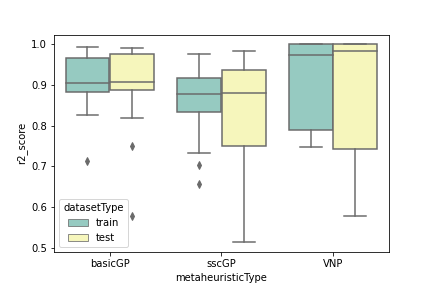
\includegraphics[width=1.1\linewidth]{../images/f1.png}
  \captionof{figure}{$F_{1}$}
  \label{fig:f1}
\end{minipage}%
\begin{minipage}{.5\textwidth}
  \centering
  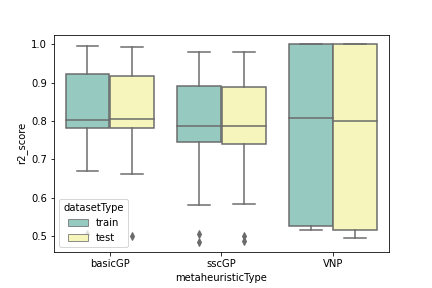
\includegraphics[width=1.1\linewidth]{../images/f2.png}
  \captionof{figure}{$F_{2}$}
  \label{fig:f2}
\end{minipage}
\end{figure}


\begin{figure}
\centering
\begin{minipage}{.5\textwidth}
  \centering
  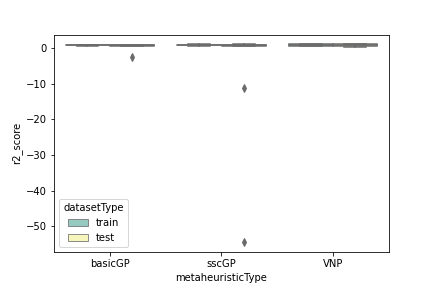
\includegraphics[width=1.1\linewidth]{../images/f3.png}
  \captionof{figure}{$F_{3}$}
  \label{fig:f3}
\end{minipage}%
\begin{minipage}{.5\textwidth}
  \centering
  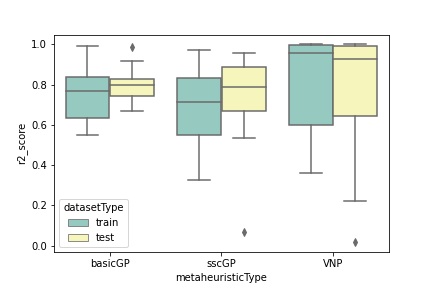
\includegraphics[width=1.1\linewidth]{../images/f4.png}
  \captionof{figure}{$F_{4}$}
  \label{fig:f4}
\end{minipage}
\end{figure}


\begin{figure}
\centering
\begin{minipage}{.5\textwidth}
  \centering
  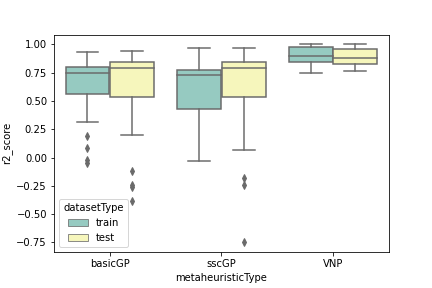
\includegraphics[width=1.1\linewidth]{../images/f5.png}
  \captionof{figure}{$F_{5}$}
  \label{fig:f5}
\end{minipage}%
\begin{minipage}{.5\textwidth}
  \centering
  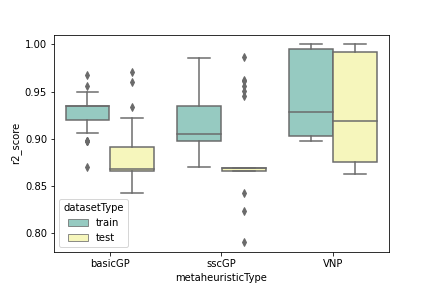
\includegraphics[width=1.1\linewidth]{../images/f6.png}
  \captionof{figure}{$F_{6}$}
  \label{fig:f6}
\end{minipage}
\end{figure}


\begin{figure}
\centering
\begin{minipage}{.5\textwidth}
  \centering
  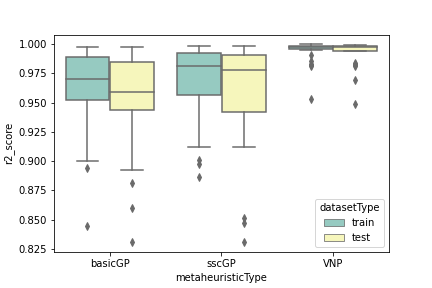
\includegraphics[width=1.1\linewidth]{../images/f7.png}
  \captionof{figure}{$F_{7}$}
  \label{fig:f7}
\end{minipage}%
\begin{minipage}{.5\textwidth}
  \centering
  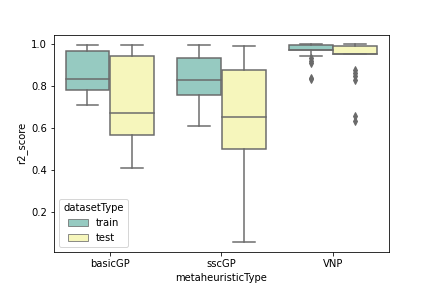
\includegraphics[width=1.1\linewidth]{../images/f8.png}
  \captionof{figure}{$F_{8}$}
  \label{fig:f8}
\end{minipage}
\end{figure}


\begin{figure}
\centering
\begin{minipage}{.5\textwidth}
  \centering
  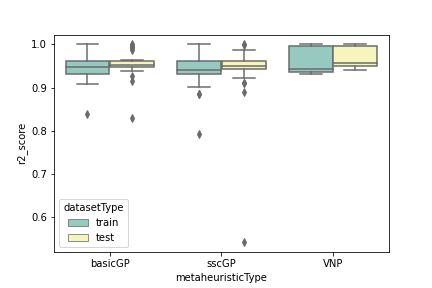
\includegraphics[width=1.1\linewidth]{../images/f9.png}
  \captionof{figure}{$F_{9}$}
  \label{fig:f9}
\end{minipage}%
\begin{minipage}{.5\textwidth}
  \centering
  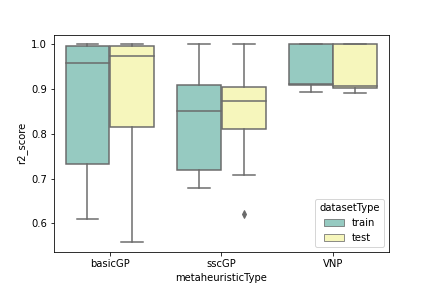
\includegraphics[width=1.1\linewidth]{../images/f01.png}
  \captionof{figure}{$F_{01}$}
  \label{fig:f01}
\end{minipage}
\end{figure}


\begin{figure}
\centering
\begin{minipage}{.5\textwidth}
  \centering
  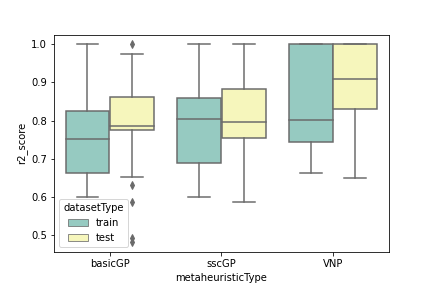
\includegraphics[width=1.1\linewidth]{../images/f02.png}
  \captionof{figure}{$F_{02}$}
  \label{fig:f02}
\end{minipage}%
\begin{minipage}{.5\textwidth}
  \centering
  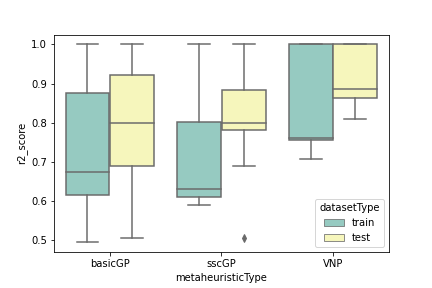
\includegraphics[width=1.1\linewidth]{../images/f03.png}
  \captionof{figure}{$F_{03}$}
  \label{fig:f03}
\end{minipage}
\end{figure}

\begin{figure}
\centering
\begin{minipage}{.5\textwidth}
  \centering
  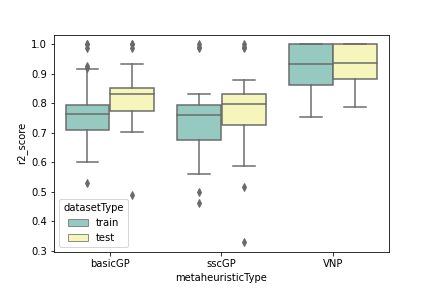
\includegraphics[width=1.1\linewidth]{../images/f04.png}
  \captionof{figure}{$F_{04}$}
  \label{fig:f04}
\end{minipage}%
\begin{minipage}{.5\textwidth}
  \centering
  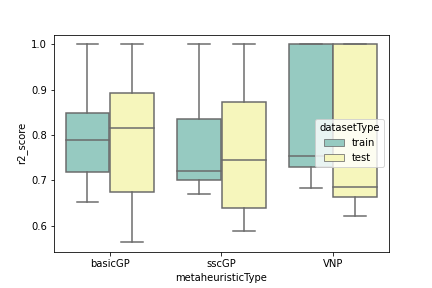
\includegraphics[width=1.1\linewidth]{../images/f05.png}
  \captionof{figure}{$F_{05}$}
  \label{fig:f05}
\end{minipage}
\end{figure}


\begin{figure}[!ht]
\begin{center}
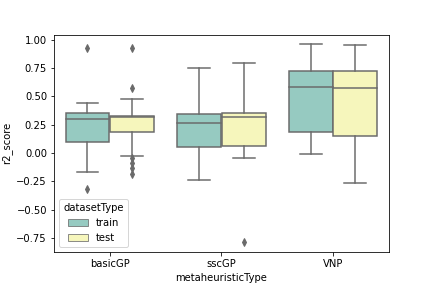
\includegraphics[width=0.9\textwidth]{../images/yacht_hydrodynamics.png}
\end{center}
\caption{\textit{Yacht Hydrodynamics}}
\label{fig:yacht}
\end{figure}


\end{document}